\documentclass[a4paper,11pt]{article}

%-------------------- PACKAGES --------------------%
\usepackage[top=0.3in, bottom=0.3in, left=0.4in, right=0.4in]{geometry} % Page margins
\usepackage{hyperref} % For clickable links
\usepackage{enumitem} % Customizable list environments
\usepackage{xcolor} % Color text and links
\usepackage{graphicx} % To include images
\usepackage{titlesec} % Custom section titles
\usepackage{fontspec} % Custom fonts
\usepackage{fontawesome} % For icons
\setlength{\parindent}{0pt} % To Remove Indentation in title

%-------------------- HYPERLINK SETUP --------------------%
\hypersetup{
    colorlinks=true,
    linkcolor=blue,
    filecolor=magenta,
    urlcolor=cyan,
    pdftitle={Abhigyan Bafna Resume},
    pdfpagemode=FullScreen,
}

%-------------------- LIST ITEM SETUP --------------------%
% Customize itemize environment for compactness
\setlist[itemize]{leftmargin=1.5em, topsep=0pt, itemsep=2pt, parsep=0pt}

%-------------------- TITLE FORMATTING --------------------%
% Adjust section title styles and spacing
\titleformat{\section}{\LARGE\bfseries}{\thesection}{1em}{}[\titlerule]
\titlespacing*{\section}{0pt}{*1.5}{*1.5}

%-------------------- CUSTOM COMMANDS --------------------%
% Entry for work experience, projects, etc. with name and date
\newcommand{\entry}[2]{
  \noindent\textbf{#1}\hfill{#2}\\[-1em]
}

% For adding hyperlinks with styled text
\newcommand{\contactlink}[2]{
    \href{#1}{\color{cyan}\underline{#2}}
}

% Environment for itemized lists with custom padding
\newenvironment{itemizeWithPadding}{
  \begin{itemize}
}{
  \end{itemize}
  \vspace{0.5em} % Bottom padding adjustment for lists
}

%-------------------- FONT SETUP --------------------%
% Main font: Roboto (Regular, Bold, Italic)
\setmainfont{Roboto}[
    Path = ./fonts/Roboto/,
    Extension = .ttf,
    UprightFont = *-Regular,
    BoldFont = *-Bold,
    ItalicFont = *-Italic,
]

% Thin version of Roboto
\newfontface\robothin{Roboto-Thin}[
    Path = ./fonts/Roboto/,
    Extension = .ttf
]

% Font for headings: Glacial Indifference
\newfontfamily\headingfont{GlacialIndifference}[
    Path = ./fonts/GlacialIndifference/,
    Extension = .otf,
    UprightFont = *-Regular,
    ItalicFont = *-Italic,
    BoldFont = *-Bold
]

%-------------------- DOCUMENT BEGINS --------------------%
\begin{document}

% Header with name and contact info
\begin{minipage}{0.87\textwidth}
{\headingfont\textbf{\huge ABHIGYAN BAFNA}}\\[0.5em]
\faEnvelope\,\contactlink{mailto:abhigyanbafna7@gmail.com}{abhigyanbafna7@gmail.com} \ | \
\faGlobe\,\contactlink{https://abhigyan.tech}{Website} \ | \
\faLinkedinSquare\,\contactlink{https://www.linkedin.com/in/AbhigyanBafna}{LinkedIn} \ | \
\faGithub\,\contactlink{https://github.com/AbhigyanBafna}{GitHub}\\[0.5em]
\textit{An engineering undergraduate with a knack for solving problems\\and building new things.}
\end{minipage}
\hfill
\begin{minipage}{0.13\textwidth}
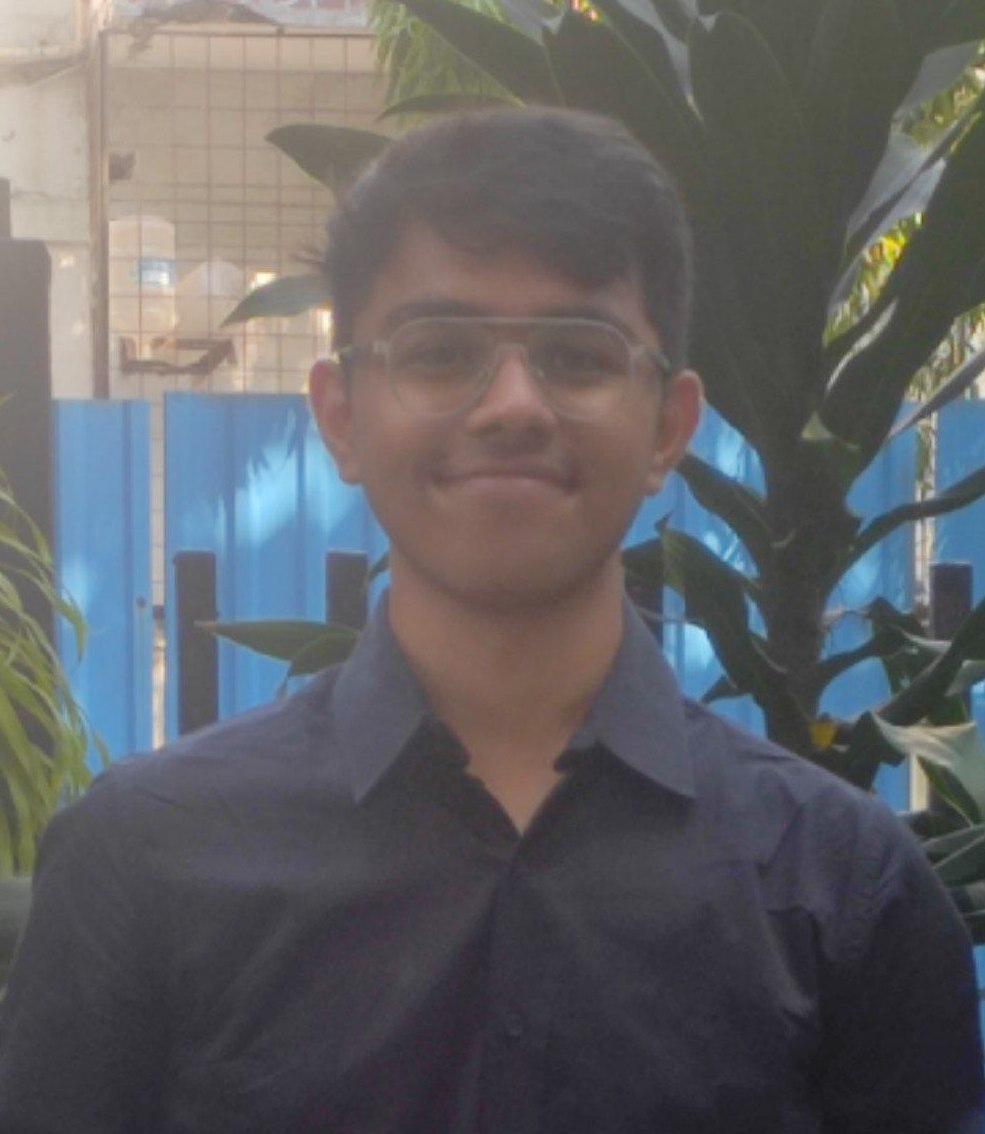
\includegraphics[width=2.5cm]{profilePicture.jpg}
\end{minipage}

%-------------------- WORK EXPERIENCE --------------------%
\section*{WORK EXPERIENCE}

\entry{\contactlink{https://www.theagentic.ai/}{TheAgenticAI} | AI Engineer}{Oct 2024 - Present}
\begin{itemizeWithPadding}
  \item Built multiple vertical AI agents like \contactlink{https://github.com/TheAgenticAI/TheAgenticBrowser}{TheAgenticBrowser.} A multi-system AI agent that can run concurrent web navigation or research based tasks.
  \item Led multiple 0-1 client project developments, managing ideation to deployment with cross-functional teams.
\end{itemizeWithPadding}

\entry{\contactlink{https://www.generalmills.co.in/}{General Mills} | Summer Internship}{June 2024}
\begin{itemizeWithPadding}
  \item Developed an API automation system for shipment activities at a Fortune 500 FMCG leader, reducing operational costs by 40-60\%.
  \item Implemented scalable backend solutions to streamline logistics and supply chain processes.
\end{itemizeWithPadding}

\entry{\contactlink{https://simppl.org/}{SimPPL} | Research Fellowship}{June 2024}
\begin{itemizeWithPadding}
  \item Contributed to misinformation combat research at Stanford-affiliated group.
  \item Worked on research and development of data pipelines for systems to detect and counter targeted hate speech and harassment against public figures.
\end{itemizeWithPadding}

%-------------------- PROJECTS --------------------%
\section*{PROJECTS}

\entry{\contactlink{https://seismo.abhigyan.tech}{Seismo} | Chrome Extension}{}
\begin{itemizeWithPadding}
  \item A Chrome extension that monitors web requests and provides instant color-coded notifications of errors across the web.
  \item Features AI-powered error analysis, privacy-first design, and dev-friendly debugging tools.
\end{itemizeWithPadding}

\entry{\contactlink{https://abhigyan.tech/blog}{ARC} | Web App}{}
\begin{itemizeWithPadding}
  \item A full-stack engineered personal blog that has a custom RTE, headless CMS, and follows ISR.
\end{itemizeWithPadding}

\entry{\contactlink{https://asthenic.vercel.app/}{Asthenic} | Aesthetic photo sharing built with React + Sanity.}{} 

\entry{\contactlink{https://github.com/AbhigyanBafna/Synopsize}{Synopsize} | AI-powered content summarization tool.} 


%-------------------- SKILLS --------------------%
\section*{SKILLS}
\vspace{-1.25em}
\begin{minipage}{0.3\textwidth}
    \begin{itemize}
        \item \textbf{Programming Languages:}
        \item \textbf{Frameworks/Libraries:}
        \item \textbf{Databases:}
        \item \textbf{Miscellaneous:}
    \end{itemize}
\end{minipage}
\begin{minipage}{0.7\textwidth}
    \vspace{1.75em}
    \setlength{\baselineskip}{1.2\baselineskip}  % Increase line spacing for clarity
     \textbf{Python}, {Javascript}, Java\\
     \textbf{NextJS}, MERN Stack, Sanity.io\\
     \textbf{MongoDB}, PostgreSQL\\
     \textbf{Google Apps Script}, AWS, GCP, MuleSoft\\    
\end{minipage}
\vspace{-2em}

%-------------------- EDUCATION --------------------%
\section*{EDUCATION}

\entry{Thadomal Shahni Engineering College | Mumbai University | B.E (I.T)}{June 2025}
% \begin{itemizeWithPadding}
%   \item Passed Semester 8 with 8.70 CGPI.
% \end{itemizeWithPadding}

\entry{Pace Junior Science College | 12th MSBSHSE (90.5\%)}{July 2021}

\entry{Gopi Birla Memorial School | 10th CBSE (93.2\%)}{May 2019}

%-------------------- OTHER ACHIEVEMENTS --------------------%
\section*{OTHER ACHIEVEMENTS}

\entry{4x Hackathon Winner | SPIT | MumbaiHacks | TSEC Hacks | TSEC Codetantra}{}\\
\entry{\href{https://ietetsec.in/}{IETE-TSEC} | Head of Technical}{2023}
\begin{itemizeWithPadding}
    \item Directed the technical department, conceptualized, and managed multiple college level events.
\end{itemizeWithPadding}

\entry{Freelance | Design \& Web}{}
\begin{itemizeWithPadding}
  \item Worked with clients around the globe, built things ranging from white label applications to designing logos and cards.
  % \href{https://rms-frontend-inky.vercel.app/}{Link.}
\end{itemizeWithPadding}

\end{document}